\documentclass{beamer}

\usepackage[utf8]{inputenc}
\usepackage{graphicx}

\usetheme{CambridgeUS}
\usecolortheme{beaver}

\title[ProbEmbed]{Generative Embedding: Learning Embeddings with Dirichlet Processes and Heavy Tails}
\author{Adith -- Chenhao -- Moontae}
\institute{Cornell}
\date{September 2014}

\begin{document}
\begin{frame}
\titlepage
\end{frame}

\begin{frame}{Learning embeddings}
  \begin{itemize}
    \item Mapping discrete atoms (words/phrases) into a continuous space
    \item Useful representation for several NLP tasks \cite{Turian}
  \end{itemize}
\begin{figure}[h!]
  \caption{Discovering implicit relationships between words \cite{CBOW}}
  \centering
    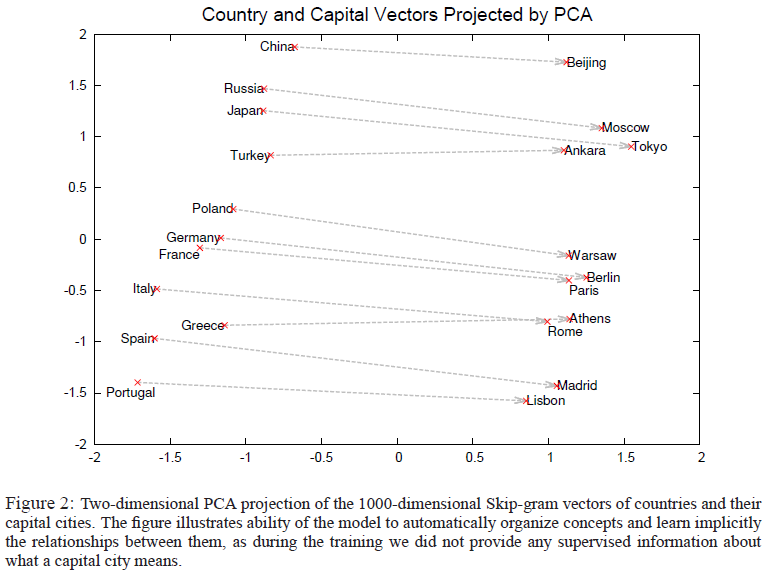
\includegraphics[width=0.5\textwidth]{CBOW.png}
\end{figure}
\end{frame}

\begin{frame}{An utter and incomplete history of embeddings}
  \begin{itemize}
    \item Distributional hypothesis \cite{Lillian}
    \item Generative Topic Models \cite{LDA}
    \item SENNA \cite{Collobert}
    \item WordReprs \cite{Turian}
    \item NCE \cite{Mnih}
    \item Multi-prototype \cite{Socher}
    \item CBOW/Skip-gram \cite{CBOW}
  \end{itemize}
\end{frame}

\begin{frame}{Goal}
Hopefully, generative models also recover good performance of existing embeddings in other settings.
\end{frame}

\begin{frame}{Why generative models?}
  \begin{itemize}
    \item Learning problem is well specified
    \item Modular models for adding complexity/assumptions
    \item Embedding quality aligned with learning objective
  \end{itemize}
\end{frame}

\begin{frame}{Formal specification}
  \begin{block}{Notation}
    $D$: all observations\\
    $X$: word embeddings
  \end{block}
  \begin{block}{Bayesian framework}
    $Pr(X)$: prior\\
    $Pr(D | X)$: likelihood
  \end{block}
  \begin{block}{Problem}
    Learning: $X^* = argmax_{ X } Pr(X | D) = argmax_{ X } Pr(X) \cdot Pr(D | X)$\\
    Evaluation: $Pr(D_{heldout}|X^*)$
  \end{block}
\pause
What other evaluations should we do \& who to compare against?
\end{frame}

\begin{frame}{DP Means prior}
  \begin{block}{Model our intuition on concept clustering in the prior}
  \end{block}
\end{frame}

\begin{frame}{Replacement game}
  \begin{block}{Model heavy tail distributions}
    $$Pr(w_j|w_i, X) = \frac{\frac{1}{1+(X_i-X_j)^2}}{\sum_{w}\frac{1}{1+(X_w-X_i)^2}}$$
  \end{block}
  \pause
  \begin{block}{Learning problem}
    $$argmin_{X, \mu, z, k} -\sum_{i}\sum_{j}Pr(w_j|w_i, X)+\lambda(\sum_i|||X_i-\mu_{z_i}|_2^2 + \sigma k)$$
  \end{block}
\end{frame}

\begin{frame}{Preliminary experiments with song embeddings from playlists}
\end{frame}

\begin{frame}{Questions?}
  \begin{itemize}
    \item Replacement game, generation game or other likelihood?
    \item Can we actually evaluate based on generative story?
    \item What other evaluations should we do \& who to compare with?
  \end{itemize}
\end{frame}

\begin{frame}[allowframebreaks]{References}
  \bibliographystyle{amsalpha}
  \bibliography{ProbEmbed}
\end{frame}

\end{document}